\documentclass[10pt]{article}
%	options include 12pt or 11pt or 10pt
%	classes include article, report, book, letter, thesis

\usepackage[a4paper,bindingoffset=0.2in,%
left=1in,right=1in,top=0.2in,bottom=0.3in,%
footskip=.15in]{geometry}

\usepackage[T1]{fontenc}
\usepackage[polish]{babel}
\usepackage[utf8]{inputenc}
\usepackage{lmodern}
\usepackage{pgfplots}
\usepackage{graphicx}
\usepackage{amsmath}
\usepackage{subcaption}
\usepackage{multirow}
\usepackage{hyperref}
\usepackage{mathtools}
\newtheorem{hip}{Hipoteza}
\newtheorem{que}{Pytanie}
\newtheorem{wn}{Wniosek}
\newtheorem{wyd}{Zadanie}
\title{Algorytmy numeryczne}
\author{Zadanie 3 \\ Dawid Bińkuś \& Oskar Bir \& Mateusz Małecki\\grupa 1 tester-programista}
\date{9 Grudzień 2018}

\begin{document}
\maketitle 

\section{Majority/Consensus problem}
Sprawozdanie prezentuje analizę problemu przeprowadzenia głosowania większościowego, przedstawionego w sposób następujący:\\
Dane jest $N$ agentów, o trzech możliwych stanach: $\{Y,N,U\}$, znaczące kolejno: agent głosujący na TAK, agent głosujący na NIE oraz agent niezdecydowany.
W każdym kroku omawianego problemu losowanych jest dwóch agentów z równomiernym prawdopodobieństwem ($\frac{2}{n\cdot (n-1)}$). Następnie dochodzi do zmiany stanu wybranych agentów według następujących reguł przejść stanów:
\begin{itemize}
	\item $\{Y,U\} \to \{Y,Y\}$,
	\item $\{Y,N\} \to \{U,U\}$,
	\item $\{N,U\} \to \{N,N\}$,
\end{itemize}
Kroki wykonywane są, dopóki wszyscy agenci nie będą jednakowego stanu.
\\
Dla danego prawdopodobieństwa $P_{\#Y,\#N}$, niech $\#N$ oznacza ilość agentów głosujących na NIE, a $\#Y$ ilość agentów głosujących na TAK.
Program przygotowany w ramach projektu, ma na celu obliczenie prawdopodobieństwa zagłosowania na TAK przy liczbie agentów równej $N$ i określonym stanie początkowym. Do jego obliczenia wykorzystany został układ równań liniowych obliczony za pomocą 3 różnych algorytmów:
\begin{itemize}
	\item Algorytm Gaussa z częściowym wyborem elementu początkowego (nazywany dalej PG) oraz jego wariant z optymalizacją dla macierzy rzadkich (nazywany dalej PGS)
	\item Algorytm Jacobiego z postacią iteracyjną:\\
	${x_{i}}^{(k+1)}=\frac{-\sum_{j=1}^{n}a_{ij}{x_j}^{k}+b_i}{a_{ii}}, i=1,2,...,n,  j\neq i.$
	\item Algorytm Gaussa-Seidela z postacią iteracyjną:\\
	${x_{i}}^{(k+1)}=\frac{-\sum_{j=1}^{i-1}a_{ij}{x_j}^{(k+1)}-\sum_{j=i+1}^{n}a_{ij}{x_j}^{(k)}+b_i}{a_{ii}}$
\end{itemize}
\section{Implementacja i możliwość stosowania metod iteracyjnych}
\begin{figure}[h]
	\caption{Wykres reprezentujący błąd bezwzględny metod Gaussa oraz metod iteracyjnych względem metody MonteCarlo\label{rys}}
	\centering
	\begin{subfigure}{0.5\textwidth}
		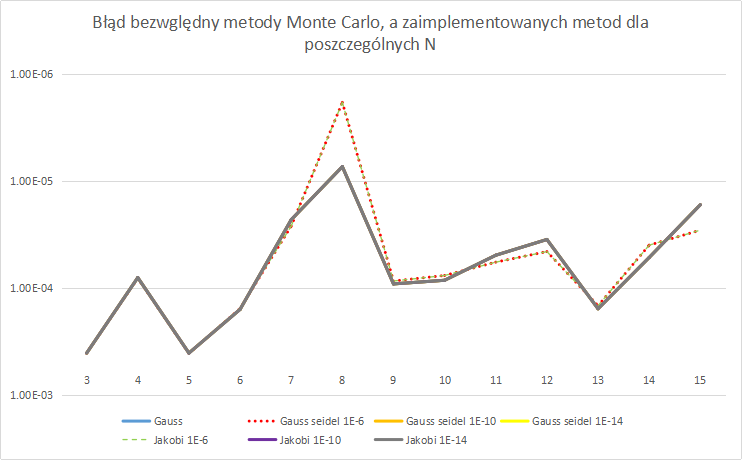
\includegraphics[width=\textwidth]{1.png}
		\caption{ \label{Rys1a}}
	\end{subfigure}
\end{figure}
\subsection{Generowanie układu równań dla danej liczby agentów}
Generowanie układu równań dla danego $N$ odbywa się w sposób następujący:
\begin{enumerate}
	\item Określenie wszystkich możliwych przypadków (ilość agentów $\#Y$ oraz ilość agentów $\#N$),
	\item Wyliczenie wszystkich możliwych kombinacji bez powtórzeń za pomocą Symbolu Newtona ${{N} \choose {2}}$,
	\item Wygenerowanie równań dla poszczególnych przypadków,
	\item Osadzenie równań w macierzy
	\item Wypełnienie wektora $B$ zerami z wyjątkiem ostatniej wartości (gdyż ostatni przypadek jest zawsze przypadkiem pewnym, tj $P_{\#Y=N,\#N=0}=1)$
\end{enumerate}
\subsection{Prawidłowość implementacji}
By zweryfikować poprawność implementacji zarówno generowania macierzy jak i obliczania stworzonego w ten sposób układu równań, wykonane zostały testy dla $N = 3,4,...,15$, których zadaniem było obliczenie wszystkich możliwych prawodopodobieństw i zestawienie ich z prawdopodobieństwem wyliczonym za pomocą metody MonteCarlo w ilości iteracji $=1000000$
Błędy osiągnięte za pomocą metod Gaussa \ref{Rys1a} osiągają wartości rzędu $1$, co biorąc pod uwagę niedoskonałość metody MonteCarlo jest wynikiem jak najbardziej zadowalającym.
\subsection{Metody iteracyjne a problem}
Wnioskując z wykresu \ref{Rys1a} możemy śmiało stwierdzić, iż metody iteracyjne są jak najbardziej słusznym sposobem na rozwiązanie problemu. Jednakże, najistotniejszym czynnikiem w przypadku ich działania jest zakładana dokładność obliczeń, tj $\|{X^{(k+1)}-X^{(k)}}\| < p$, gdzie $p$ = żądana precyzja.
W przypadku zadanej dokładności równej $10^{-6}$ zauważyć można że, różnice względem wartości wyliczonej za pomocą metody MonteCarlo są większe niż w przypadku metod iteracyjnych z większą zadaną dokładnością ($10^{-10}, 10^{-14}$).
\begin{wn}
	Metody iteracyjne umożliwiają rozwiązanie problemu aczkolwiek, by osiągnąć dokładniejsze wyniki, należy zwiększyć dokładność, a co za tym idzie - liczbę iteracji, co znacząco wydłuża czas działania algorytmu.
\end{wn}
\section{Analiza wyników i wydajność zaimplementowanych algorytmów}
\begin{figure}[h]
	\caption{Wykresy reprezentujące czas wykonania i błędy bezwzględne zaimplementowanych algorytmów \label{rys}}
	\begin{subfigure}{0.5\textwidth}
		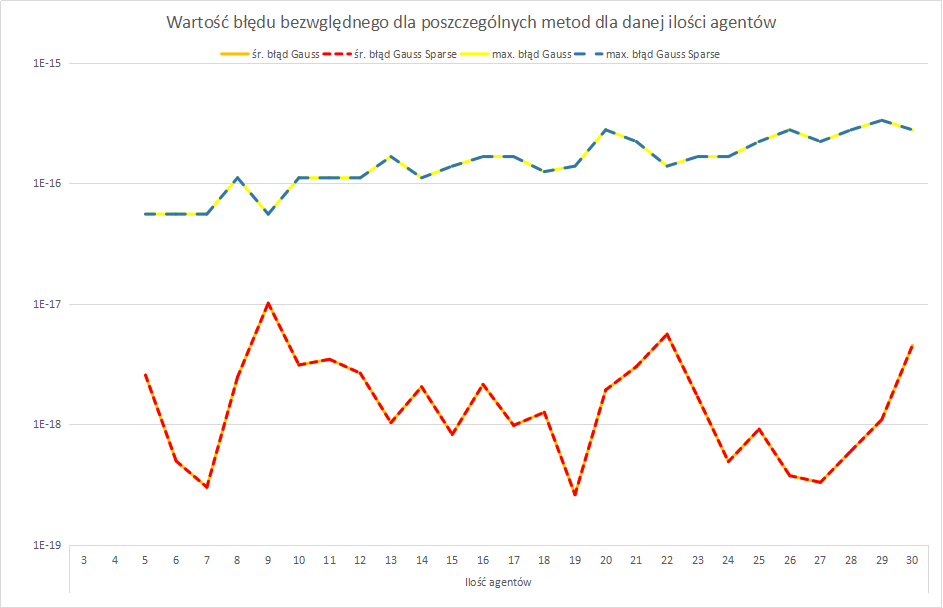
\includegraphics[width=\textwidth]{2.png}
		\caption{ \label{Rys2a}}
	\end{subfigure}
	\begin{subfigure}{0.5\textwidth}
	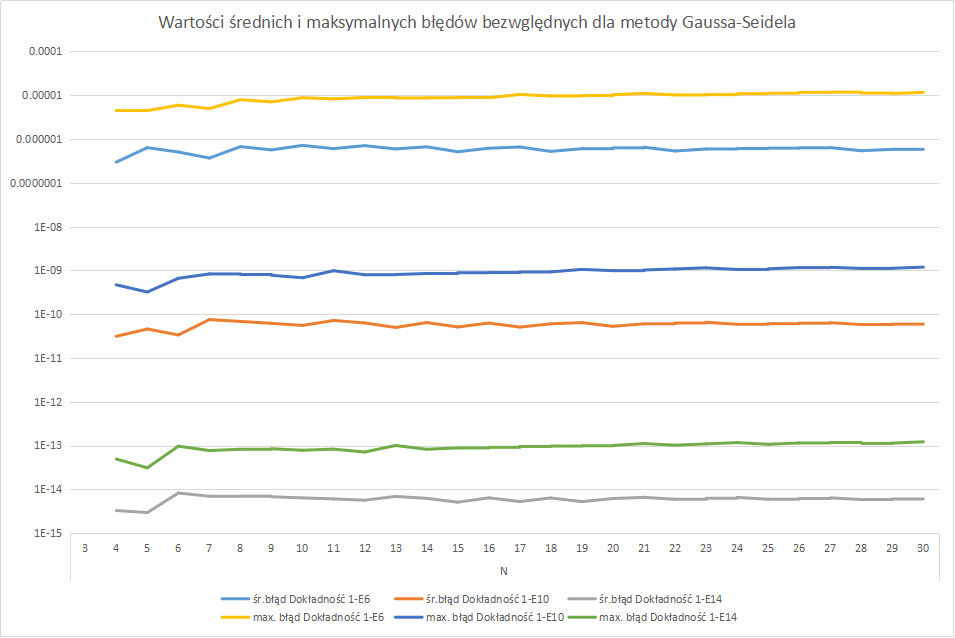
\includegraphics[width=\textwidth]{3.png}
	\caption{ \label{Rys2b}}
	\end{subfigure}
	\begin{subfigure}{0.5\textwidth}
	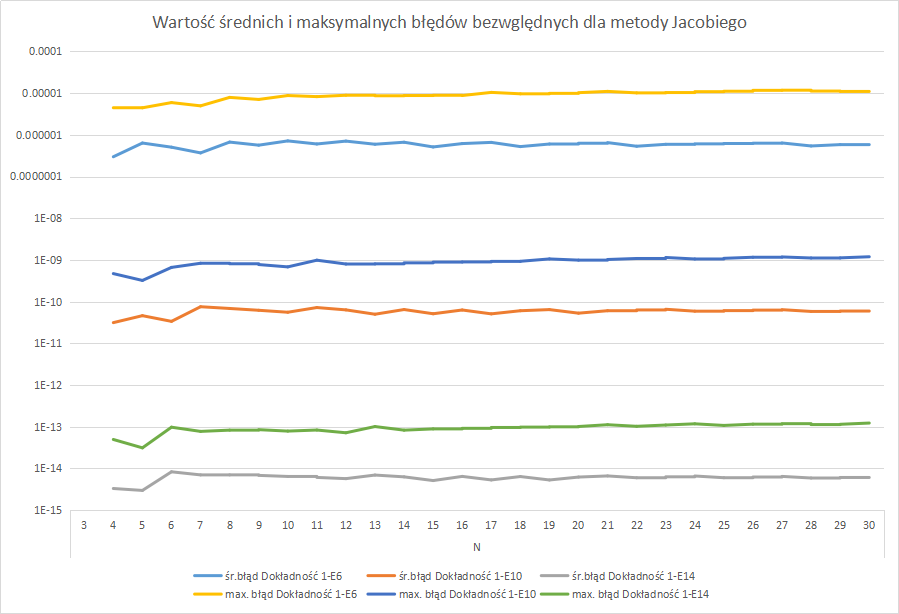
\includegraphics[width=\textwidth]{4.png}
	\caption{ \label{Rys2c}}
	\end{subfigure}
\end{figure}
\subsection{Analiza wyników}
Błąd bezwzględny dla poszczególnych metod był wyliczany w sposób następujący:
\begin{enumerate}
	\item Wygenerowana została macierz $A$ oraz wektor $B$
	\item Za pomocą danego algorytmu obliczany zostaje wektor $X$ (wynikowy)
	\item Wykonujemy operację $A\cdot x = b'$
	\item Wyliczany jest błąd bezwzględny kolejnych wartości wektora $b'$ względem wektora $b$
	\item Jako błąd przechowywana jest największa wartość oraz jej średnia
\end{enumerate}
\subsubsection{Gauss oraz Gauss z optymalizacją dla macierzy rzadkich}
Przeanalizujmy wykres \ref{Rys2a}. Zostało na nim przedstawione zestawienie wyników dla wartości średniej oraz maksymalnej błędu bezwzględnego. Z wartości na nich ukazanych wynika, że w przypadku metod PG oraz PGS, zarówno maksymalny jak i średni błąd jest identyczny.
\begin{wn}
	Algorytm PG oraz PGS osiągają taką samą dokładność. Dodanie optymalizacji dla macierzy rzadkich nie ma żadnego wpływu na końcowy wynik.\label{wn:1}
\end{wn}
\subsubsection{Algorytmy iteracyjne}
Przeanalizujmy wykresy \ref{Rys2b} oraz \ref{Rys2c}. Prezentują one maksymalny oraz średni błąd bezwzględny dla różnej zadanej dokładności: $10^{-6},10^{-10}$ oraz $10^{-14}$.
Wnioski z nich są następujące:
\begin{wn}
	Zarówno algorytm Jacobiego jak i Gaussa-Seidela oferują taką samą dokładność, w zależności od tego jaka precyzja była żądana. Warunek kończący iterowanie był zależny od maksymalnego błędu między kolejnymi iteracjami - stąd mniejszy średni błąd bezwzględny. \label{wn:2}
\end{wn}
\subsection{Wydajność}
\subsubsection{Metody PG oraz PGS}
Przeanalizujmy wykres XD. Zauważyć na nim można znaczną przewagę algorytmu PGS względem PG w czasie wykonywania. Wynika to ze specyfiki działania wariantu PGS - algorytm ten pomija redukcję elementów w wierszu w przypadku gdy wybrany na początku element jest równy zeru.
\begin{wn}
	Wariant PGS algorytmu Gaussa jest wydajniejszy niż standardowy wariant PG. Zestawiając ten wniosek z wnioskiem \ref{wn:3} stwierdzić można, iż wariant PGS zapewnia o wiele lepszą wydajność nie mając żadnego wpływu na poprawność zwracanych wyników
	 \label{wn:3}
\end{wn}
\subsubsection{Metody iteracyjne}
W przypadku metod iteracyjnych, należy rozważyć osobno algorytmy dla różnej zadanej precyzji.
Jednakże we wszystkich przypadków, zależność jest następująca: Metoda Gaussa-Seidela w każdym przypadku (wraz z wzrostem $N$) ma krótszy czas wykonania względem metody Jacobiana.
\begin{wn}
	Metoda Gaussa-Seidela jest wydajniejsza od metody Jacobiana - wynika to ze sposobu działania obu tych algorytmów. Metoda Jacobiana by osiągnąć żądaną precyzję musi wykonać o wiele więcej iteracji niż metoda Gaussa-Seidela. \label{wn:4}
\end{wn}
\subsection{Podsumowanie}
\begin{wn}
	XD
\end{wn}
\section{Podział pracy}
\centering
	\begin{tabular}{| p{5cm} | p{5cm} | p{5cm} |}
		\hline
		\textbf{Dawid Bińkuś} & \textbf{Oskar Bir} & \textbf{Mateusz Małecki} \\ \hline
		Implementacja algorytmu PG oraz PGS & Implementacja algorytmu Gaussa-Seidela & Implementacja algorytmu Jacobiego \\ \hline
		Przygotowanie sprawozdania & Przygotowanie testów i ich uruchomienie & Praca nad strukturą projektu \\ \hline
		Implementacja algorytmu generowania macierzy & Przygotowanie wykresów końcowych &Implementacja symulacji MonteCarlo\\ \hline
		
		
		
	\end{tabular}
\end{document}